%!TEX root = ../NCVC7.tex
\mysection{仕上げ等高線のNCデータを生成}

\subsection{仕上げ等高線用スキャニングパスの生成}
 仕上げ用のデータを生成するには,切削対象となるNURBS曲面を1つ選択する必要があります.
マウスの左クリックで選択してください.

 NURBS曲面が選択されていると,\menu{ファイル>NCデータの生成>仕上げ等高線パスの生成}(\keys{F3})のメニューが有効になります.
図~\ref{fig:ncvc31} のダイアログから適当な値を設定してください.

\begin{figure}[H]
\centering
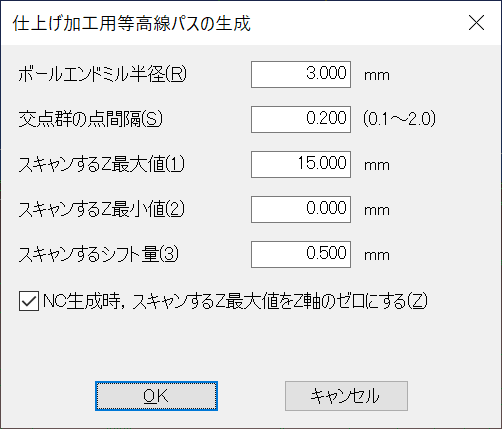
\includegraphics{No3/fig/fig31.png}
\caption{仕上げ加工用等高線パスの生成}
\label{fig:ncvc31}
\end{figure}

 荒加工データの生成からシミュレーション結果を表示するところまで作業していたとすると,

\begin{itemize}
\item \keys{F6}(ウィンドウの切り替え)でIGESデータのウィンドウにする.
\item \keys{F3}(仕上げ等高線パスの生成)で 図~\ref{fig:ncvc31} を表示(NURBS曲面が選択状態のはず).
\item \keys{F7}(3D切削データの生成)でNCデータを出力.
\end{itemize}

のようにショートカットキーを駆使して効率よく作業を進めることが可能です.

\vspace*{1zh}
 図~\ref{fig:ncvc31} で \keys{OK} を押すと,しばらく計算したあと,図~\ref{fig:ncvc32} のように仕上げ用の等高線パスが表示されます.
この等高線はNURBS曲面上に点群がプロットされます.
裏面を見ても 図~\ref{fig:ncvc33} のように点群が貫通して見えますが気にしないでください
\footnote{ポリゴンオフセットという手法で面を少しだけずらして描画しています.こうしないと表面であっても「zファイティング」と言われる不自然なレンダリング結果になります.}.

\begin{figure}[H]
\centering
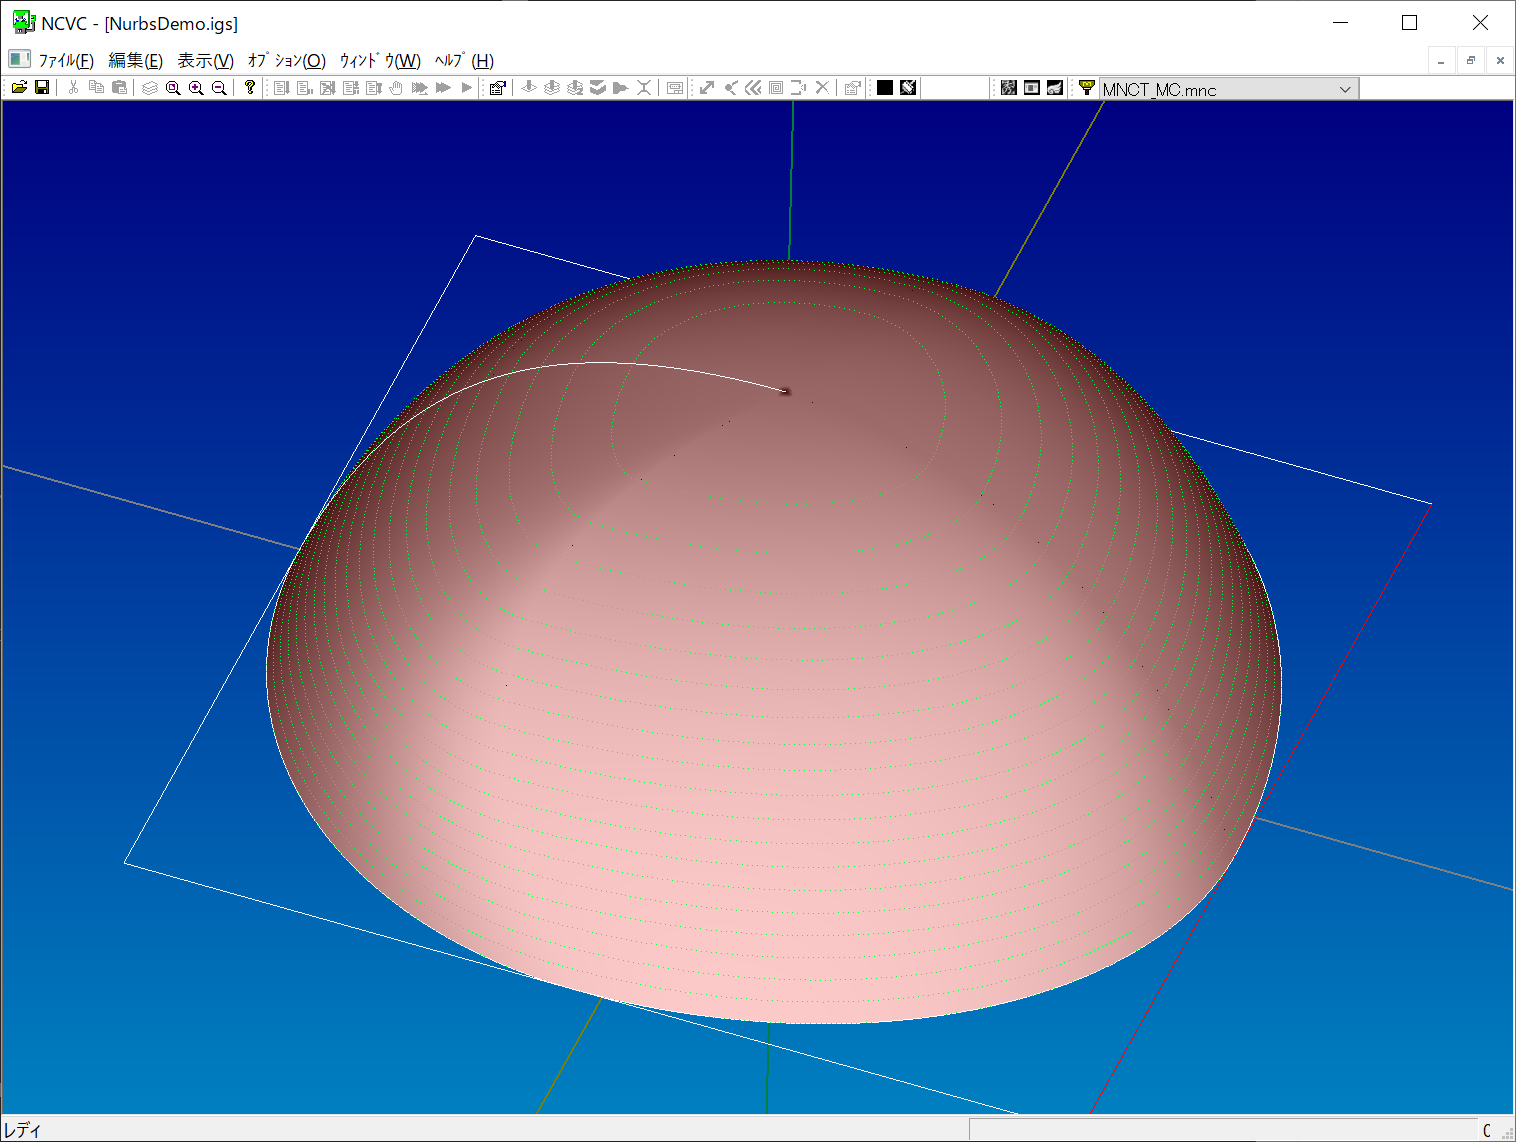
\includegraphics[scale=0.5]{No3/fig/fig32.png}
\caption{仕上げスキャニングパスの表示}
\label{fig:ncvc32}
\end{figure}

\begin{figure}[H]
\centering
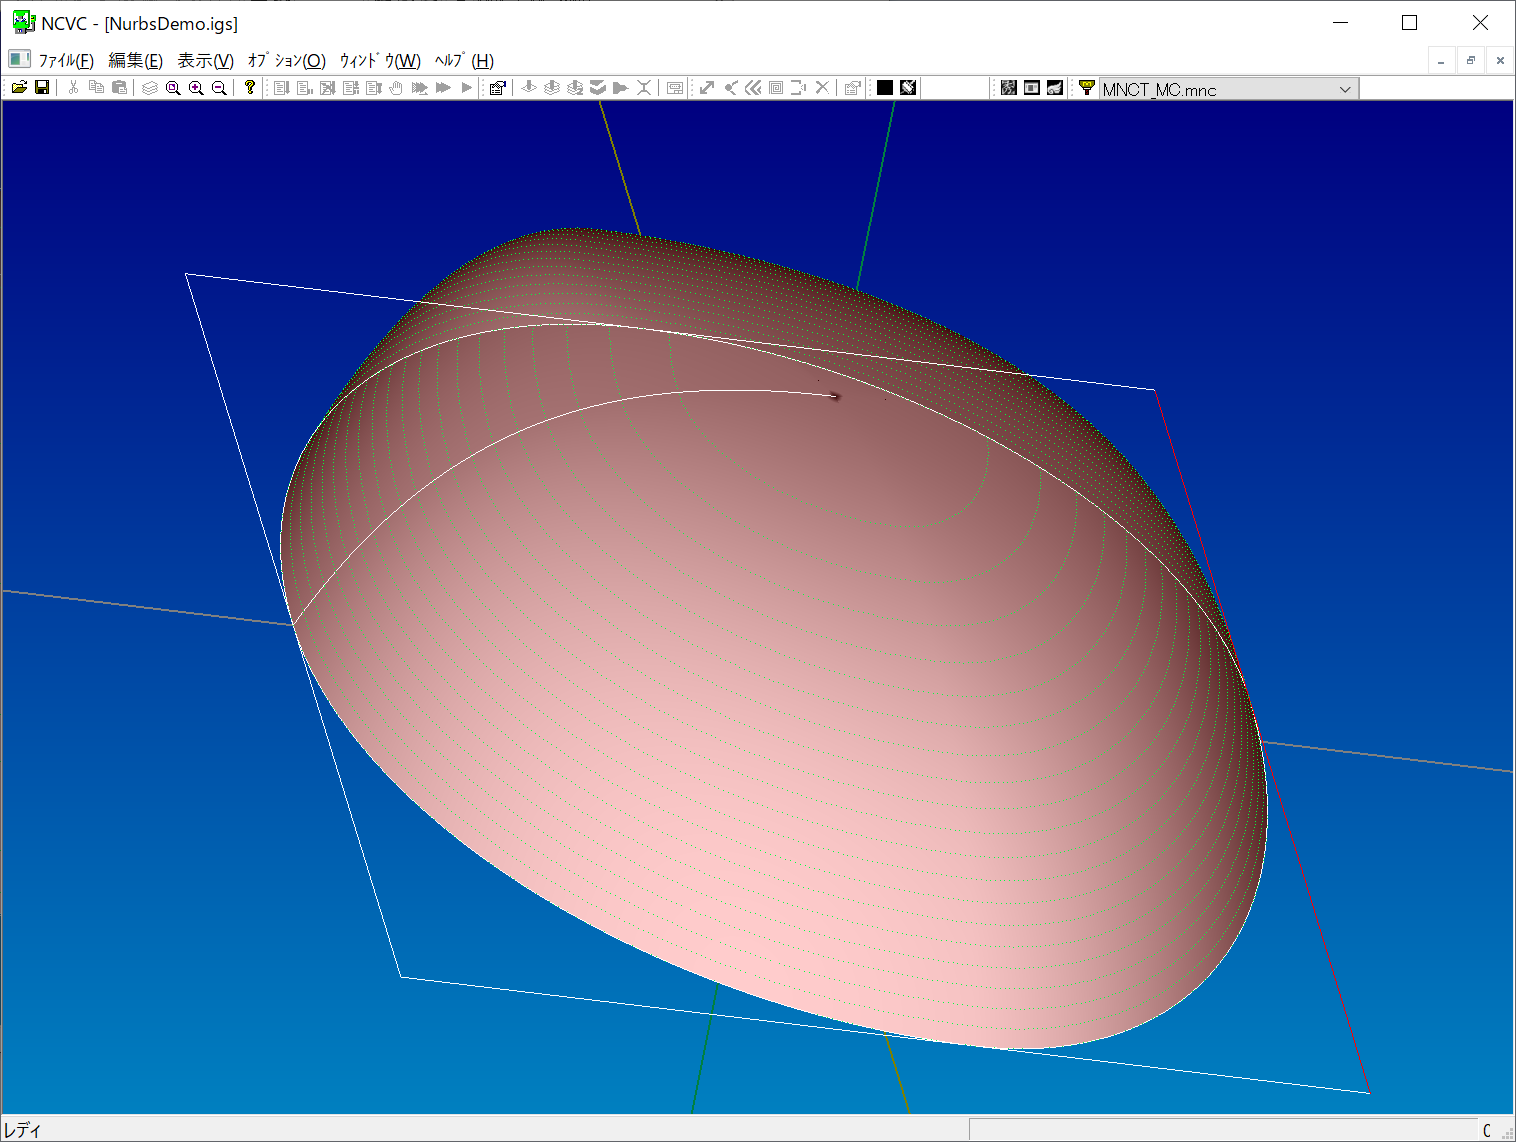
\includegraphics[scale=0.5]{No3/fig/fig33.png}
\caption{裏面のようす}
\label{fig:ncvc33}
\end{figure}

\newpage
\subsection{NCデータの出力とシミュレーション結果}
 荒加工と同じように \menu{ファイル>NCデータの生成>3D切削データの生成}(\keys{F7})のメニューから出力できます.
出力ファイル名にはデフォルトで仕上げ加工用の \_Contour というサフィックス(接尾語)が付けられます(図~\ref{fig:ncvc34}).
切削条件は 図~\ref{fig:ncvc27} と同じなので省略します.

\begin{figure}[H]
\centering
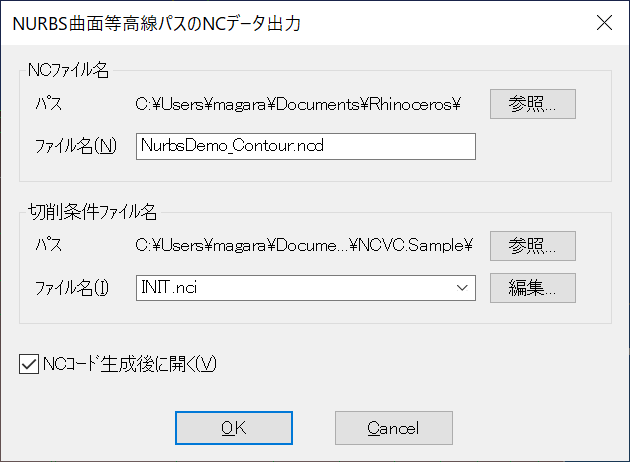
\includegraphics[scale=0.7]{No3/fig/fig34.png}
\caption{仕上げ加工用NCデータの出力設定}
\label{fig:ncvc34}
\end{figure}

 荒加工と同じようにエンドミル情報が自動的に埋め込まれるので,図~\ref{fig:ncvc35}のように生成後即正確な切削イメージがシミュレーションできます.

\begin{figure}[H]
\centering
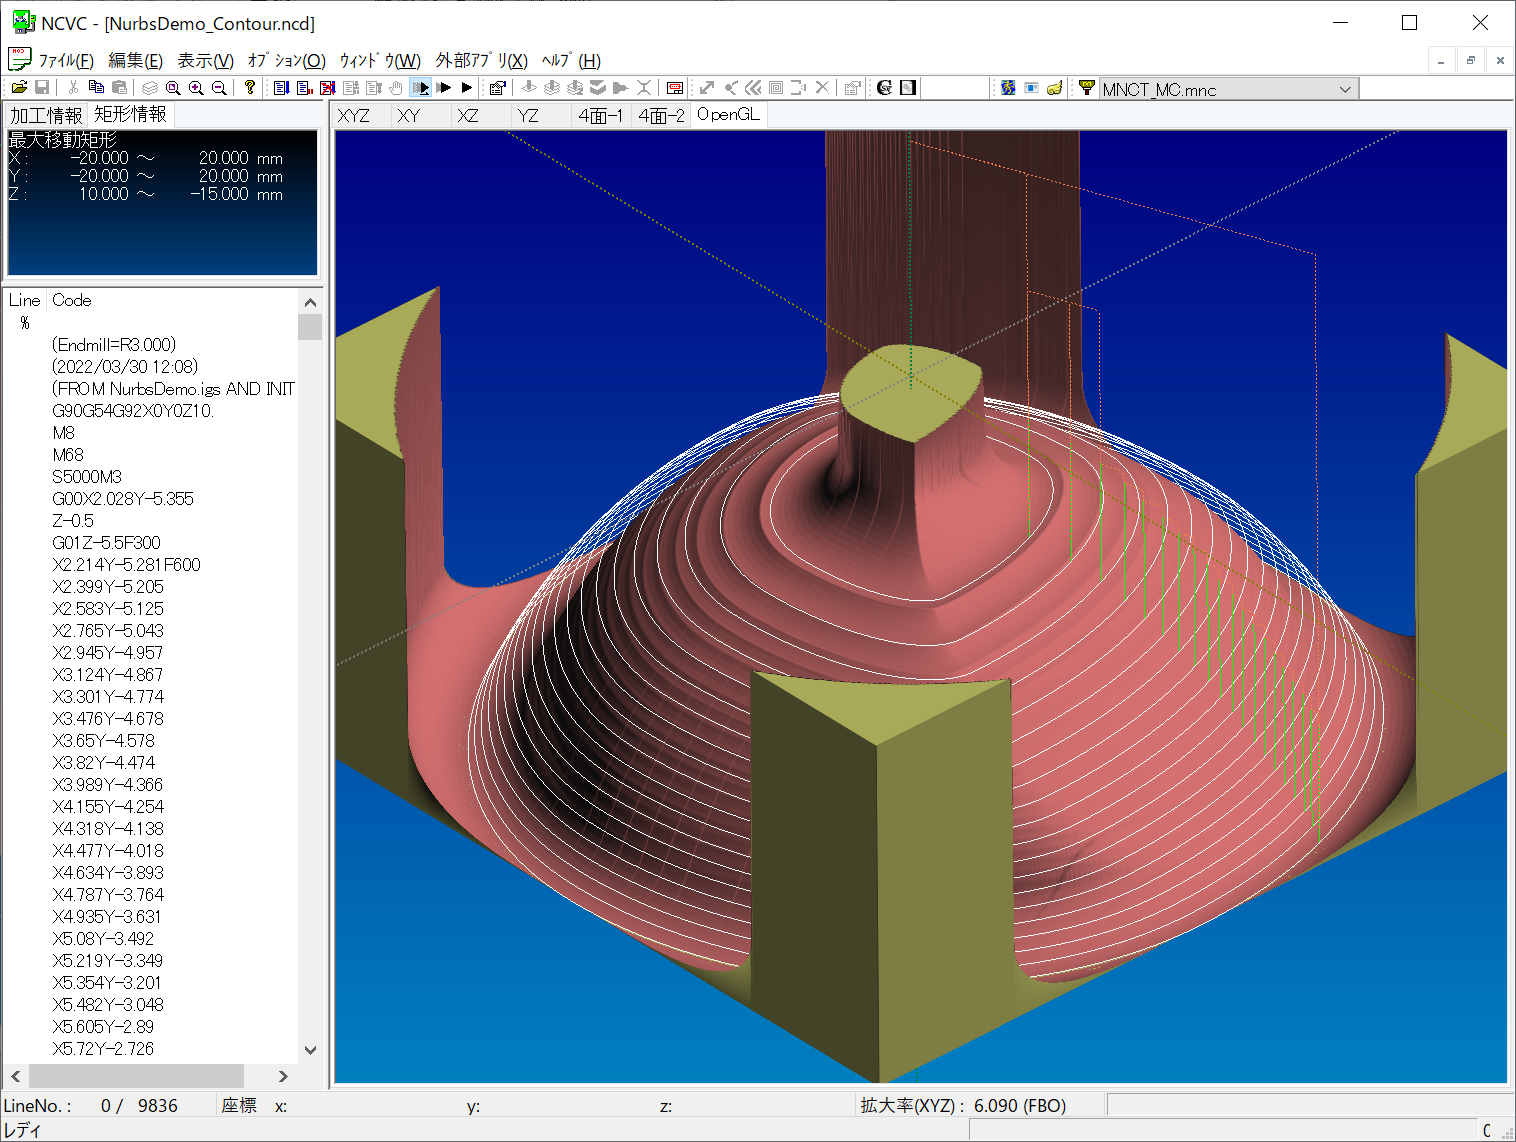
\includegraphics[scale=0.5]{No3/fig/fig35.png}
\caption{仕上げ等高線NCデータのシミュレーション結果}
\label{fig:ncvc35}
\end{figure}


%\vspace*{3zh}
\newpage
\begin{itembox}[l]{ここまでの【まとめ】}
(1) IGESデータ
\begin{itemize}
\item NURBSの曲線と曲面のみ
\item NCVCが落ちる場合もある
\item 読めない場合はIGESタイプを変更
\end{itemize}
(2) 荒加工
\begin{itemize}
\item NURBSのガイド曲線と曲面を選択
\item \keys{F2}$\rightarrow$\keys{F7} でシミュレーション確認
\item ダメなら\keys{F6}$\rightarrow$ガイド曲線を変える$\rightarrow$\keys{F7}
\end{itemize}
(2) 仕上げ
\begin{itemize}
\item NURBSの曲面を選択
\item \keys{F3}$\rightarrow$\keys{F7} でシミュレーション確認
\end{itemize}
\end{itembox}
